\documentclass[a4paper,12pt]{article}

\usepackage[utf8]{inputenc}
\usepackage[T2A]{fontenc}
\usepackage[russian]{babel}
\usepackage{amsmath, amssymb}
\usepackage{geometry}
\usepackage{graphicx}
\usepackage[hidelinks]{hyperref}

\geometry{margin=2cm}

\usepackage[most]{tcolorbox}

\usepackage{fancyhdr}

\pagestyle{fancy}

\fancyhf{} 

\fancyhead[L]{ФИЗИКА. ЭКЗАМЕН. 2-й СЕМЕСТР}
\fancyhead[R]{АРТЁМ КИМ ИУ7-22Б}

\fancyfoot[C]{\thepage} 

\newtcolorbox{definitionbox}{
colback=white,
colframe=green!60!black,
boxrule=0pt,
leftrule=3pt,
rightrule=0pt,
toprule=0pt,
bottomrule=0pt,
left=6pt,
right=0pt,
top=3pt,
bottom=3pt
}

\newtcolorbox{theorembox}{
colback=white,
colframe=red!70!pink,
boxrule=0pt,
leftrule=3pt,
rightrule=0pt,
toprule=0pt,
bottomrule=0pt,
left=6pt,
right=0pt,
top=3pt,
bottom=3pt
}

\begin{document}

\tableofcontents

\section{Кинематика основ механики}

\subsection*{1. Радиус-вектор, перемещение, скорость, ускорение материальной точки и связь между ними. (РК1 - 1)}

\subsection*{План}
\begin{itemize}
\item Дать определение радиус-вектора
\item Ввести перемещение и его модуль
\item Получить выражение мгновенной скорости как производной радиус-вектора
\item Получить выражение ускорения как производной скорости
\item Разложить ускорение на касательную и нормальную составляющие
\item Вывести формулы через производную единичного касательного вектора
\end{itemize}
    
\begin{definitionbox}
\textbf{Радиус-вектор} — вектор, задающий положение точки относительно начала координат.
\end{definitionbox}

\begin{definitionbox}
\textbf{Вектор перемещения} $\Delta \vec R$ за интервал $(t_1, t_2)$ — вектор, соединяющий начальное и конечное положение точки.
\end{definitionbox}

\[
\Delta \vec R
=
\vec R(t_2)
-
\vec R(t_1)
=
(x_2-x_1,\; y_2-y_1,\; z_2-z_1)
\]

\[
|\Delta \vec R|
=
\sqrt{(\Delta x)^2 + (\Delta y)^2 + (\Delta z)^2}
\]

\begin{definitionbox}
\textbf{Мгновенная скорость} $\vec v$ — предел средней скорости при $\Delta t \to 0$.
\end{definitionbox}

\[
\vec v
=
\lim_{\Delta t \to 0}
\frac{\Delta \vec R}{\Delta t}
\]

\[
\vec v
=
\dot{\vec R}(t)
\]

\begin{definitionbox}
\textbf{Мгновенное ускорение} $\vec a$ — предел изменения скорости при $\Delta t \to 0$.
\end{definitionbox}

\[
\vec a
=
\lim_{\Delta t \to 0}
\frac{\Delta \vec v}{\Delta t}
=
\dot{\vec v}(t)
=
\ddot{\vec R}(t)
\]

Вектор ускорения можно разложить на две составляющие:

\[
\vec a
=
\vec a_{\tau}
+
\vec a_n
\]

\begin{definitionbox}
$\vec a_{\tau}$ — тангенциальное (касательное) ускорение.
\end{definitionbox}

\begin{definitionbox}
$\vec a_n$ — нормальное ускорение.
\end{definitionbox}

Введём единичный вектор:

\[
\vec \tau_v
=
\frac{\vec v}{|\vec v|}
\]

Тогда

\[
\vec v
=
\vec \tau_v |\vec v|
\]

Найдём ускорение:

\[
\vec a
=
\frac{d\vec v}{dt}
=
\frac{d}{dt}\left(\vec \tau_v |\vec v|\right)
\]

\[
\vec a
=
\underbrace{
\left(\frac{d\vec \tau_v}{dt}\right) |\vec v|
}_{\text{нормальное}}
+
\underbrace{
\vec \tau_v \left(\frac{d|\vec v|}{dt}\right)
}_{\text{тангенциальное}}
\]

Рассмотрим нормальную часть.

Пусть $d\varphi$ — малый угол поворота касательной к траектории; 
$\vec n$ — единичный нормальный вектор; 
$ds$ — малый элемент длины дуги траектории.

\[
\frac{d\vec \tau_v}{dt}
=
\vec{n}\frac{d\varphi}{dt}
=
\frac{\vec{n}}{R}\frac{ds}{dt}
=
\frac{\vec n}{R} |\vec v|
\]

\[
\vec a
=
\vec \tau_v \frac{d|\vec v|}{dt}
+
\vec n \frac{|\vec v|^2}{R}
\]

\[
a_\tau
=
\frac{d|\vec v|}{dt},
\qquad
a_n
=
\frac{|\vec v|^2}{R}
\] 

\subsection*{2. Линейная скорость и ускорение твёрдого тела при вращательном движении. Связь угла поворота, угловой скорости и углового ускорения. Связь угловой скорости с линейной. Все аналитические выражения необходимо вывести (РК1 - 2)}

\textbf{План}
\begin{itemize}
\item Ввести угловую скорость
\item Ввести угловое ускорение
\item Найти связь линейной скорости с угловой
\item Найти ускорение при вращении
\item Разложить ускорение на касательную и нормальную составляющие
\item Связь угловых величин с периодом и частотой
\item Связь линейных и угловых величин
\end{itemize}

\begin{definitionbox}
\textbf{Угловая скорость} $\vec \omega$ — векторная величина, характеризующая скорость изменения угла поворота тела.  (направлена вдоль оси вращения)
\end{definitionbox}

\[
\vec \omega
=
\frac{d\vec \varphi}{dt}
=
\dot{\varphi}
\]

\[
[\omega] = \text{рад/с}
\]

\begin{definitionbox}
\textbf{Угловое ускорение} $\vec \varepsilon$ — векторная величина, характеризующая скорость изменения угловой скорости.
\end{definitionbox}

\[
\vec \varepsilon
=
\frac{d\vec \omega}{dt}
=
\dot{\omega}
=
\ddot{\varphi}
\]

\[
[\varepsilon] = \text{рад/с}^2
\]

Рассмотрим радиус-вектор точки:

\[
\vec r
=
\vec r_\parallel + \vec r_\perp
\]

\begin{figure}[h]
\centering
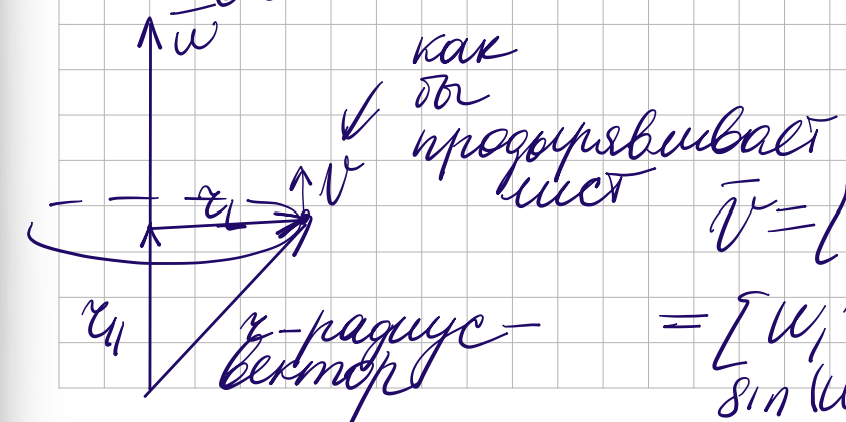
\includegraphics[width=0.5\textwidth]{trajectory.png}
\caption{Направления скоростей}
\end{figure}

Линейная скорость точки вращающегося тела:

\[
\vec v
=
[\vec \omega, \vec r]
\]

\[
\vec v
=
[\vec \omega, \vec r_\parallel + \vec r_\perp]
=
[\vec \omega, \vec r_\parallel]
+
[\vec \omega, \vec r_\perp]
\]

Так как

\[
\sin(\vec \omega, \vec r_\parallel)=0; 
 \sin(\vec \omega, \vec r_\perp)=1
\]

то

\[
\vec v
=
[\vec \omega, \vec r_\perp]
\]

Модуль линейной скорости:

\[
v
=
\omega r_\perp
\]

Найдём ускорение:

\[
\vec a
=
\frac{d\vec v}{dt}
=
\frac{d}{dt}[\vec \omega, \vec r_\perp]
\]

\[
\vec a
=
[\dot \vec \omega, \vec r_\perp]
+
[\vec \omega, \dot \vec r_\perp']
\]

\[
\vec a
=
\underbrace{[\vec \varepsilon, \vec r_\perp]}_{\text{тангенциальное}}
+
\underbrace{[\vec \omega, \vec v]}_{\text{нормальное}}
\]
Так как

\[
v = \omega r_\perp
\]

получаем нормальное ускорение:

\[
a_n
=
\omega^2 r_\perp
=
\frac{v^2}{r_\perp}
\]

\begin{definitionbox}
\textbf{Касательное ускорение} $\vec a_\tau$ — составляющая ускорения, направленная вдоль скорости.
\end{definitionbox}

\[
\vec a_\tau
=
[\vec \varepsilon, \vec r_\perp]
\]

\begin{definitionbox}
\textbf{Нормальное ускорение} $\vec a_n$ — составляющая ускорения, направленная к центру вращения.
\end{definitionbox}

\[
\vec a_n
=
[\vec \omega, \vec v]
\]

Полное ускорение:

\[
\vec a
=
\vec a_\tau
+
\vec a_n
\]

\begin{definitionbox}
    \textbf{Период} $T$ — время, за которое тело совершает один полный оборот.
\end{definitionbox}


\[
T
=
\frac{2\pi}{\omega}
\]

\[
\omega
=
\frac{2\pi}{T}
\]


\begin{definitionbox}
    \textbf{Частота} $\nu$ — физическая величина, равная числу полных оборотов за единицу времени.
\end{definitionbox}
\[
\nu
=
\frac{1}{T}
\]

\[
{\omega}
=
2\pi \nu
\]
 
\subsection*{Классический закон сложения скоростей и ускорений при поступательном движении подвижной системы отсчёта}

План:
\begin{itemize}
\item Рассмотреть две системы отсчёта
\item Ввести радиус-векторы точки в разных системах
\item Получить связь радиус-векторов
\item Вывести закон сложения скоростей
\item Вывести закон сложения ускорений
\item Ввести сопутствующую систему отсчёта
\end{itemize}
 

\begin{definitionbox}
Поступательное движение — движение, при котором оси системы отсчёта остаются параллельными самим себе, вращение отсутствует.
\end{definitionbox}

Рассмотрим две системы отсчёта: система 1 и система 2, движущуюся поступательно относительно первой.

Положение точки A:

в системе 1 задаётся радиус-вектором $\vec R_1$

в системе 2 задаётся радиус-вектором $\vec R_2$

Радиус-вектор начала системы 2 относительно системы 1:

$\vec R_{21}$

\begin{figure}[h]
\centering
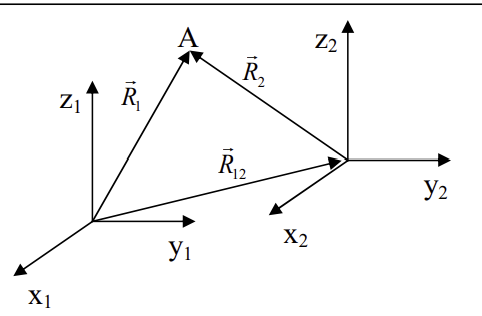
\includegraphics[width=0.5\textwidth]{ref_systems.png}
\caption{Сложение скоростей}
\end{figure}

\subsubsection*{1. Связь радиус-векторов}

По правилу сложения векторов:



\[
\vec R_2
=
\vec R_1
+
\vec R_{21}
\]

\subsubsection*{2. Закон сложения скоростей (вывод)}


\[
\vec v_2
=
\frac{d\vec R_2}{dt}
\]

Подставим выражение для радиус-вектора:

\[
\vec v_2
=
\frac{d}{dt}
\left(
\vec R_1
+
\vec R_{21}
\right)
\]

\[
\vec v_2
=
\frac{d\vec R_1}{dt}
+
\frac{d\vec R_{21}}{dt}
\]

Обозначим:

\[
\vec v_1
=
\frac{d\vec R_1}{dt}
\]

\[
\vec v_{21}
=
\frac{d\vec R_{21}}{dt}
\]

где $\vec v_{21}$ — скорость системы 2 относительно системы 1 (вроде бы)

Получаем:

\[
\vec v_2
=
\vec v_1
+
\vec v_{21}
\]

\subsubsection*{3. Закон сложения ускорений (вывод)}
 

\[
\vec a_2
=
\frac{d\vec v_2}{dt}
\]

\[
\vec a_2
=
\frac{d}{dt}
\left(
\vec v_1
+
\vec v_{21}
\right)
\]

\[
\vec a_2
=
\frac{d\vec v_1}{dt}
+
\frac{d\vec v_{21}}{dt}
\]

Обозначим:

\[
\vec a_1
=
\frac{d\vec v_1}{dt}
\]

\[
\vec a_{21}
=
\frac{d\vec v_{21}}{dt}
\]

Получаем:

\[
\vec a_2
=
\vec a_1
+
\vec a_{21}
\]

\subsubsection*{4. Сопутствующая система отсчёта}

\begin{definitionbox}
Системой отсчета, сопутствующей
данной точке называется такая система отсчета, в которой вектор скорости данной точки является нулевым (т.е. точка покоится в данной системе отсчета). 
\end{definitionbox}

\[
\vec v = 0
\]

\subsection*{Понятие инерциальной системы отсчета. I, II и III законы Ньютона. Сила упругости
(закон Гука), сила тяжести (закон всемирного тяготения), сила трения скольжения
и сила сопротивления среды. (РК1 - 3) }

\textbf{План}
\begin{itemize}
\item Понятие инерциальной системы отсчёта
\item I закон Ньютона
\item II закон Ньютона (векторная и импульсная форма)
\item Принцип относительности Галилея
\item III закон Ньютона
\item Основные силы классической механики
\end{itemize}

\vspace{0.8em}

\begin{definitionbox}
\textbf{Инертность тела} — свойство тела не изменять вектор своей скорости в отсутствие внешних сил.
\end{definitionbox} 

\begin{definitionbox}
\textbf{Масса тела} — мера инертности тела.
\end{definitionbox}

В классической физике:
\begin{itemize}
\item масса аддитивна (масса системы равна сумме масс её частей.)
\item масса не зависит от системы отсчёта
\end{itemize}

Экспериментально установлено:
\[
m_{\text{инерт}} = m_{\text{грав}}
\]

\vspace{0.8em}

\textbf{I закон Ньютона}

\begin{theorembox}
pСуществуют такие системы отсчёта, в которых материальная точка либо покоится, либо движется по прямой с постоянной скоростью, если на неё не действуют силы или их векторная сумма равна нулю. Такие системы называются \textbf{инерциальными}.
\end{theorembox}

\[
\sum \vec F = 0
\;\Rightarrow\;
\vec v = const
\]
 

\vspace{0.8em}

\textbf{II закон Ньютона}

\begin{theorembox}
В инерциальной системе отсчёта ускорение материальной точки сонаправлено с вектором суммы сил, действующих на точку. Величина ускорения прямо пропорциональна равнодействующей сил и обратно пропорциональна массе точки.
\end{theorembox}

\[
\sum \vec F = m \vec a
\]

Эквивалентная форма:

\[
\vec a = \frac{\sum \vec F}{m}
\]

Проекции второго закона Ньютона:

\[
\begin{cases}
m a_x = \sum F_x \\
m a_y = \sum F_y \\
m a_z = \sum F_z
\end{cases}
\]

Импульс:

\[
\vec p = m \vec v
\]

Производная по времени:

\[
\frac{d\vec p}{dt}
=
\frac{d(m\vec v)}{dt}
\]

при постоянной массе:

\[
\frac{d\vec p}{dt}
=
m \frac{d\vec v}{dt}
\]

\[
\frac{d\vec p}{dt}
=
m \vec a
\]

по второму закону Ньютона:

\[
\frac{d\vec p}{dt}
=
\sum \vec F
\]

\vspace{0.8em}

\textbf{Принцип относительности Галилея}

\begin{theorembox}
При переходе между инерциальными системами отсчёта ускорение материальной точки не изменяется, поэтому второй закон Ньютона имеет одинаковый вид во всех инерциальных системах отсчёта.
\end{theorembox}

\[
\vec a_2 = \vec a_1
\]

\[
m \vec a = \sum \vec F
\]

\vspace{0.8em}

\textbf{III закон Ньютона}

\begin{theorembox}
Две материальные точки действуют друг на друга силами, одинаковыми по величине и противоположными по направлению.
\end{theorembox}

\[
\vec F_{12} = - \vec F_{21}
\]

Силы:
\begin{itemize}
\item лежат на одной прямой
\item приложены к разным телам
\end{itemize}

\vspace{0.8em}

\textbf{Сила всемирного тяготения}

\begin{theorembox}
Две материальные точки притягиваются с силой, пропорциональной произведению их масс и обратно пропорциональной квадрату расстояния между ними.
\end{theorembox}

\[
F
=
G \frac{m_1 m_2}{R^2}
\]

\[
G \approx 6.67 \cdot 10^{-11}
\ \text{Н·м}^2/\text{кг}^2
\]

Силы направлены вдоль прямой, соединяющей точки.

Для однородных шаров расстояние измеряется между центрами.

\vspace{0.8em}

\textbf{Сила тяжести}

Для тела массы $m$ вблизи поверхности Земли:

\[
F
=
G
\frac{M_{\text{Земли}} m}{(R_{\text{Земли}}+h)^2}
\]

если $h \ll R_{\text{Земли}}$:

\[
R_{\text{Земли}} + h \approx R_{\text{Земли}}
\]

вводим обозначение:

\[
g
=
G
\frac{M_{\text{Земли}}}{R_{\text{Земли}}^2}
\]

\[
F = mg
\]

Сила направлена к центру Земли.

\vspace{0.8em}

\textbf{Сила трения скольжения}

Сила трения возникает между соприкасающимися телами при их относительном движении.

Сила направлена против движения.

\[
F_{\text{тр}} = \mu N
\]

где:

$\mu$ — коэффициент трения скольжения

$N$ — сила нормальной реакции опоры

В классической механике сила трения не зависит от площади соприкасающихся поверхностей.

\vspace{0.8em}

\textbf{Сила сопротивления среды}

При движении тела в жидкости или газе возникает сила сопротивления.

Сила направлена против скорости тела относительно среды.

Общий вид:

\[
\vec F = - \alpha S v^n \vec e_v
\]

где:

$S$ — площадь поперечного сечения

$v$ — скорость

$\alpha$ — коэффициент среды

При малых скоростях:

\[
\vec F = - r \vec v
\]

где r > 0 - коэффициент сопротивления

\vspace{0.8em}

\textbf{Сила упругости (закон Гука)}

Деформация:

\[
x = L_1 - L
\]

\begin{theorembox}
Сила упругости, возникающая при малой деформации, прямо пропорциональна величине деформации и направлена противоположно ей.
\end{theorembox}

\[
\vec F = -k \vec x
\]

$k$ — коэффициент жёсткости.

\vspace{0.8em}

\textbf{Обобщённый закон Гука}

\begin{definitionbox}
\textbf{Напряжение (нормальное напряжение)} [Па] — в сечении отношение величины силы к площади поперечного сечения
\end{definitionbox}

\[
\sigma = \frac{F}{S}
\]

\[
F_{\text{упр}} = \sigma S = k\,\Delta L = k\,L_0 \cdot \frac{\Delta L}{L_0},
\qquad
\text{откуда }
\sigma
=
\frac{k\,L_0}{S}\cdot\frac{\Delta L}{L_0}.
\]

Относительная деформация:

\[
\varepsilon = \frac{\Delta L}{L_0}
\]

Коэффициент упругости материала или модуль Юнга [Па]:

\[
E = \frac{k L_0}{S}
\]

\begin{theorembox}
Напряжение прямо пропорционально относительной деформации.
\end{theorembox}

\[
\sigma = E \varepsilon
\]

\end{document}